% Supplementary numerical experiments.
% Required packages: amsmath, booktabs, graphicx, and xcolor.
% Figure paths are relative to this file's directory.

\begingroup
\color{blue}
\setlength{\emergencystretch}{2em}

\section{Additional Numerical Results}
\label{app:additional-experiments}

We examine how coordinate heterogeneity, dependence, calibration size, noise
tails, and residual transformations affect the coverage and efficiency of
TSCP. Comparisons with the population oracle and the unenclosed local union
separate the statistical and computational effects of its approximations.
Real-data marginal coverage and search-regime measurements complement the
results in Section~\ref{sec:numerical-experiments}.

\subsection{Additional Noise-Distribution Experiments}
\label{app:additional-distribution-experiments}
\label{app:simulations}

Tables~\ref{tab:gaussian-heter}--\ref{tab:gamma} report coverage and
normalized residual-space volume for five noise laws. Gaussian errors
contrast unequal and equal coordinate scales; Laplace, mixture, and Gamma
errors vary the tail shape and symmetry under heterogeneous scaling.
The Laplace distributions are centered at zero, with the stated scale
parameter; the Gamma parameterization specifies shape followed by scale.

\subsubsection*{Gaussian Noise (Heterogeneous)}

\begin{table}[H]
    \centering
    \input{figures/baselines/gaussian_10d_table}
    \caption{Performance with $d=10$ outcome variables, as in
    Figure~\ref{fig:gaussian-heter}. Results are averaged over 200 repetitions,
    with one standard deviation in parentheses. The target coverage is $0.9$;
    estimates below this target are highlighted in \textcolor{red}{red}.
    Bold values indicate the smallest mean residual-space volume among
    TSCP, Point CHR, and Unscaled Max. TSCP has the smallest volume among
    these methods in the displayed settings.}
    \label{tab:gaussian-heter}
\end{table}

\clearpage
\subsubsection*{Gaussian Noise (Homogeneous)}

\begin{table}[H]
    \centering
    \input{figures/baselines/unit_gaussian_10d_table}
    \caption{Performance with $d=10$ outcome variables and homogeneous
    Gaussian noise, as in Figure~\ref{fig:gaussian-homo}. Other details are
    as in Table~\ref{tab:gaussian-heter}. Unscaled Max has the smallest
    volume among methods with near-nominal coverage, while TSCP remains competitive.}
    \label{tab:gaussian-homo}
\end{table}

\clearpage
\subsubsection*{Laplace Noise}
\begin{table}[H]
    \centering
    \input{figures/baselines/laplace_10d_table}
    \caption{Performance of the proposed TSCP method and alternative conformal prediction approaches on simulated data with $d=10$ outcome variables, and noise following a \emph{Laplace} distribution; i.e., $\epsilon _j \sim \mathrm{Laplace}(10-j+1)$ for all $j \in [10]$. Other details are as in Table~\ref{tab:gaussian-heter}.}
    \label{tab:laplace}
\end{table}

\clearpage
\subsubsection*{Mixture Noise}

\begin{table}[H]
    \centering
    \input{figures/baselines/mixed_10d_table}
    \caption{Performance of the proposed TSCP method and alternative conformal prediction approaches on simulated data with $d=10$ outcome variables, and noise following a \emph{Mixture} distribution; i.e., $\epsilon_j \sim \frac{1}{2}\mathrm{Laplace}(10-j+1)+\frac{1}{2}\mathcal{N}(0, (10-j+1)^2)$ for all $j \in [10]$. Other details are as in Table~\ref{tab:gaussian-heter}.}
    \label{tab:mixed}
\end{table}

\clearpage
\subsubsection*{Gamma Noise}
 
\begin{table}[H]
    \centering
    \input{figures/baselines/gamma_10d_table}
    \caption{Performance of the proposed TSCP method and alternative conformal prediction approaches on simulated data with $d=10$ outcome variables, and noise following a \emph{Gamma} distribution; i.e., $\epsilon_j \sim  \mathrm{Gamma}(1, 10-j+1)$ for all $j \in [10]$. Other details are as in Table~\ref{tab:gaussian-heter}.}
    \label{tab:gamma}
\end{table}


\clearpage
\subsection{Dependence Strength}
\label{app:dependence-sensitivity}

We vary the equicorrelation of the Gaussian noise over
$\rho\in\{0,0.3,0.6,0.9\}$ while retaining marginal standard deviations
$(10,9,\ldots,1)$ and a calibration size of $n=100$. Figure~\ref{fig:app-dependence}
shows that TSCP's empirical joint coverage is stable across different values of $\rho$. Its average
residual-space volume decreases from $6.37\times10^{10}$ at $\rho=0$ to
$9.47\times10^9$ at $\rho=0.9$. Point CHR and Unscaled Max also remain close
to the target. Emp. Copula improves as the correlation strengthens but remains
below the nominal level throughout this test. The experiment therefore does
not indicate a coverage failure of TSCP under strong equicorrelation, while
also showing that our method adapts well to varying dependence structures.

\begin{figure*}[!htbp]
  \centering
  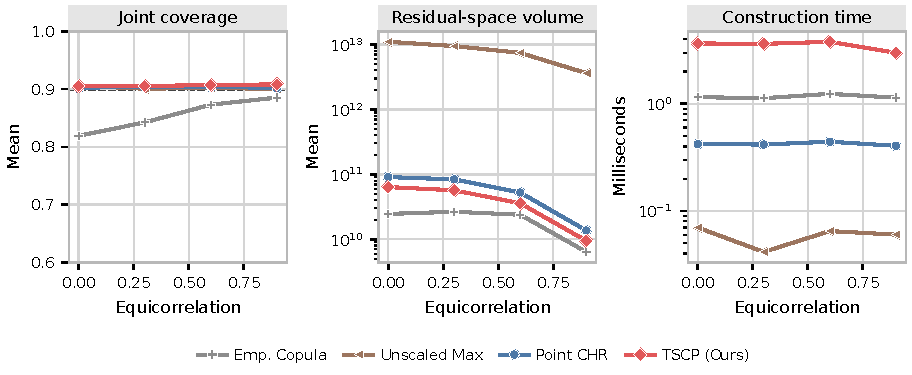
\includegraphics[width=0.92\textwidth]{figures/fig_app_dependence_sensitivity.pdf}
  \caption{Sensitivity to equicorrelated Gaussian noise at $d=10$ and
  $n=100$. The three panels report joint coverage, mean residual-space
  volume, and mean construction time. Results average 200 repetitions; the
  dashed line marks the target coverage.}
  \label{fig:app-dependence}
\end{figure*}

\subsection{Severity of Coordinate Heterogeneity}
\label{app:heterogeneity-sensitivity}

To isolate heterogeneity across outcomes, we use independent Gaussian noise
and choose ten coordinate scales geometrically spaced between $r$ and $1$,
where $r\in\{1,2,5,10,20\}$. The calibration size is fixed at $n=100$.
Figure~\ref{fig:app-heterogeneity} plots joint coverage and mean residual-space volume against the scale ratio $r$ and shows that the coverage of TSCP, Point CHR,
and Unscaled Max is essentially unchanged as $r$ grows. At $r=1$, Unscaled
Max produces slightly smaller volumes than TSCP, consistent with the
unit-scale comparison in Figure~\ref{fig:gaussian-homo}. As $r$ grows,
Unscaled Max's volume increases more steeply than the volumes of the
coordinate-adaptive methods. This widening gap
is the expected benefit of coordinate adaptation: a single maximum-residual
threshold becomes increasingly inefficient when one scale must be used for
all coordinates. 

\begin{figure*}[!htbp]
  \centering
  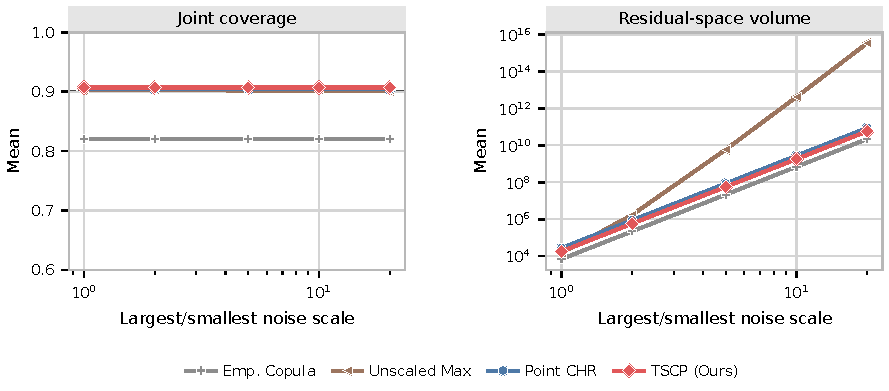
\includegraphics[width=0.84\textwidth]{figures/fig_app_heterogeneity_sweep.pdf}
  \caption{Sensitivity to the ratio between the largest and smallest outcome
  noise scales, with independent Gaussian errors and $n=100$. The scales are
  geometrically spaced, and both axes of the volume panel are logarithmic.
  Results average 200 repetitions.}
  \label{fig:app-heterogeneity}
\end{figure*}

\FloatBarrier
\subsection{Sensitivity to the Target Coverage Level}
\label{app:alpha-small-sample}

Figure~\ref{fig:app-alpha} repeats the dependent Gaussian experiment at
nominal coverage levels $0.8$, $0.9$, and $0.95$, with $n=100$ and
$\rho=0.6$. TSCP achieves empirical coverages $0.811$, $0.907$, and $0.954$.
As expected, increasing the target level increases all region volumes. The
relative ordering is stable: TSCP is smaller than Point CHR and dramatically
smaller than Unscaled Max, while Emp. Copula is smaller but below the nominal
coverage at every displayed target.

\begin{figure*}[!htbp]
  \centering
  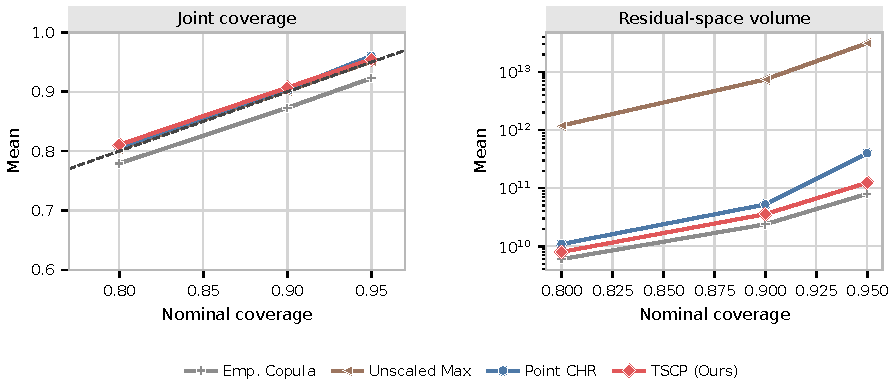
\includegraphics[width=0.84\textwidth]{figures/fig_app_alpha_sensitivity.pdf}
  \caption{Sensitivity to the nominal coverage level in the $d=10$
  equicorrelated Gaussian experiment with $n=100$ and $\rho=0.6$. The dashed
  diagonal in the left panel is exact nominal calibration. Results average
  200 repetitions.}
  \label{fig:app-alpha}
\end{figure*}

\subsection{Heavy-Tailed Noise}
\label{app:heavy-tails}

We examine independent Student $t$ noise with
$d=10$, a common unit scale across coordinates, and degrees of freedom
$\nu\in\{1.5,2,3\}$. The cases $\nu=1.5$ and $\nu=2$ have infinite variance
and therefore lie outside Assumption~\ref{eq:assumption-scores}, which is
invoked by the validity theorem as well as the moment-based motivation;
$\nu=3$ has finite variance but remains heavy-tailed.

Figure~\ref{fig:t} presents the results averaged over 200
repetitions. Coverage remains near the target while interval volumes grow
substantially as the degrees of freedom decrease. Point CHR has larger volume at the smaller calibration size but can outperform TSCP at the
larger size. 

\begin{figure}[!htbp]
     \centering
     \begin{subfigure}[b]{\textwidth}
         \centering
         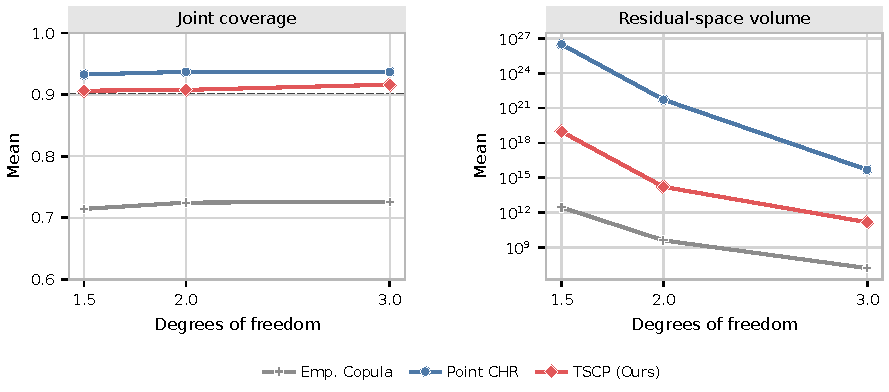
\includegraphics[width=0.9\textwidth]{figures/fig_app_heavy_tail_n30.pdf}
         \caption{Calibration size $n=30$.}
         \label{fig:t-n30-10d}
     \end{subfigure}
     \vfill
     \begin{subfigure}[b]{\textwidth}
         \centering
         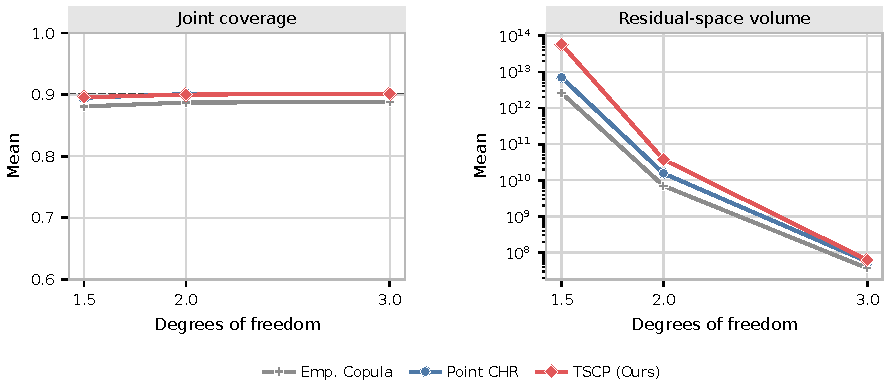
\includegraphics[width=0.9\textwidth]{figures/fig_app_heavy_tail_n500.pdf}
         \caption{Calibration size $n=500$.}
         \label{fig:t-n500-10d}
     \end{subfigure}
        \caption{Performance under Student $t$ noise with varying degrees of
        freedom, using calibration sizes (a) $n=30$ and (b) $n=500$.
        The target coverage is $0.9$. TSCP has near-nominal empirical
        coverage in these settings; the infinite-variance cases are outside
        the stated assumptions. Point CHR produces larger volumes at the
        smaller calibration size but can outperform TSCP at the larger size.
        Downward triangles at the coverage-axis boundary indicate values below $0.6$.}
        \label{fig:t}
\end{figure}

\subsection{Exchangeable Contamination Stress Test}
\label{app:contamination}

To test sensitivity to atypically large residuals, we contaminate the
Gaussian experiment at rates
$\varepsilon\in\{0,0.01,0.05,0.10\}$. Independently for each observation, all
ten noise coordinates are multiplied by $10$ with probability $\varepsilon$;
the same exchangeable mechanism is used for training, calibration, and test
data. The calibration size is $n=100$. We report median rather than mean
volume because the contaminated distribution produces a small number of
extreme regions.

Figure~\ref{fig:app-contamination} shows that TSCP coverage stays near nominal regardless of contamination, but its
median volume grows from $5.38\times10^{10}$ to $1.10\times10^{17}$. Point CHR
and Unscaled Max exhibit the same qualitative inflation, and Emp. Copula
undercovers at every contamination level. Thus, the conformal calibration is
comparatively stable in coverage, whereas the sample mean and standard
deviation used for coordinate scaling are not robust efficiency summaries.
Replacing them by robust estimators would change the construction and its
analysis and requires a separate validity argument.

\begin{figure*}[!htbp]
  \centering
  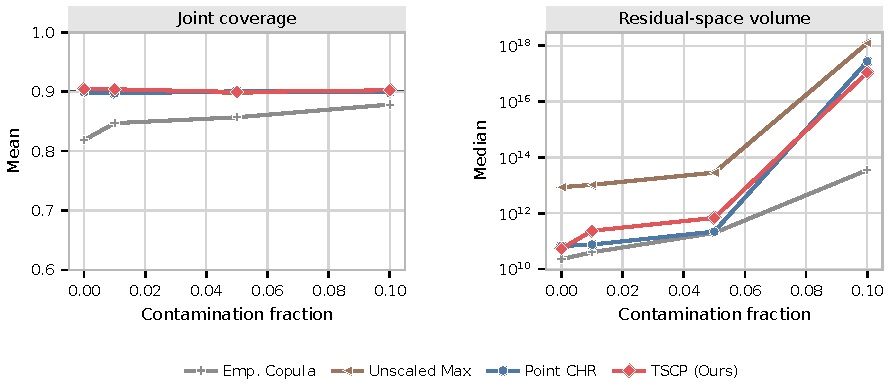
\includegraphics[width=0.84\textwidth]{figures/fig_app_contamination_stress.pdf}
  \caption{Row-wise contamination stress test with $d=10$ and $n=100$. A
  contaminated observation has every noise coordinate multiplied by $10$.
  The right panel reports median residual-space volume over 200 repetitions
  on a logarithmic scale.}
  \label{fig:app-contamination}
\end{figure*}

\FloatBarrier
\subsection{Additional CQR Sensitivity Analyses}
\label{app:cqr-sensitivity}

\paragraph{Base-interval width.}
The main CQR comparison uses base-interval miscoverage $0.5$. We repeat it at
$0.3$, $0.5$, $0.7$, and $0.9$, fixing $n=100$ and final miscoverage $0.1$.
Figure~\ref{fig:app-cqr-base} shows that TSCP with capped residuals and Unscaled Max behave
similarly, while Emp. Copula undercovers. CQHR remains close to nominal
coverage but its volume is highly sensitive to the fitted base interval in
this design.

\begin{figure*}[!htbp]
  \centering
  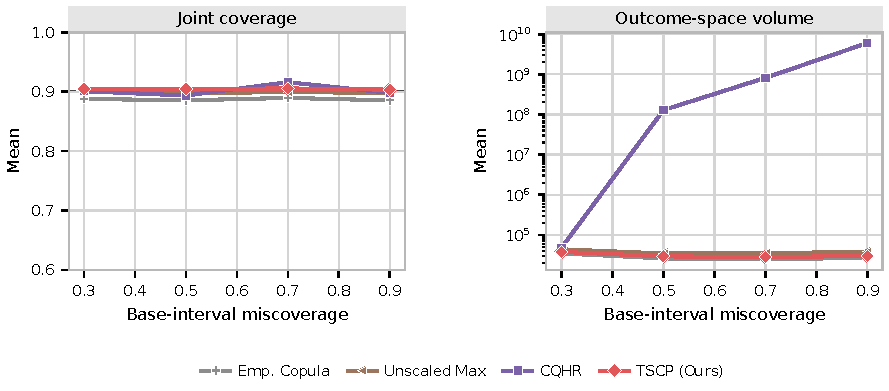
\includegraphics[width=0.84\textwidth]{figures/fig_app_cqr_base_interval.pdf}
  \caption{CQR sensitivity to the base-interval miscoverage with $d=3$,
  $n=100$, and final target coverage $0.9$. TSCP uses capped scores, CQHR uses
  its native construction, and results average 30 independent repetitions.}
  \label{fig:app-cqr-base}
\end{figure*}

\paragraph{Shifted scores.}
An alternative transformation replaces the signed CQR residuals
$E_j$ by $E_j+C$, apply TSCP, and subtract $C$ from the final coordinate
adjustment. We test $C\in\{100,300,1000\}$. As shown in
Figure~\ref{fig:app-cqr-shift}, the recorded TSCP rectangle is numerically invariant to
$C$ and, more importantly, agrees exactly with
the TSCP-GWC rectangle: the maximum coordinate-length difference is zero in
all 30 repetitions for every $C$.
% AUTHOR-CHECK SHIFT: Verify the proposed mechanism and supply a rule ensuring nonnegativity on future inputs.
The proposed explanation is that a large additive constant inflates the
LWC score bound in Section~\ref{sec:method-lwc}, so the global-worst-case
bound determines the final rectangle. Equality of the recorded rectangles
is empirical evidence, not a general shift-invariance result. Capped
residuals $\max\{E_j,0\}$ avoid choosing $C$ and are used for the main
comparison, with the limitations described in Section~\ref{sec:cqr-experiments}.

\begin{figure*}[!htbp]
  \centering
  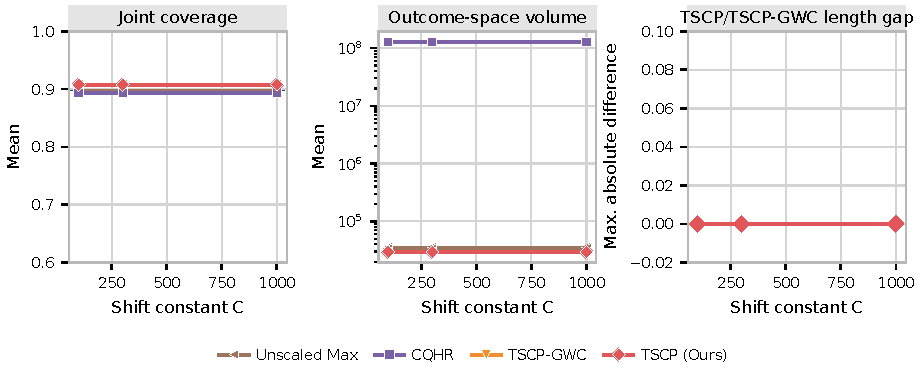
\includegraphics[width=0.92\textwidth]{figures/fig_app_cqr_shift_sensitivity.pdf}
  \caption{Sensitivity of shifted CQR scores to the additive constant $C$.
  The first two panels report coverage and mean outcome-space volume; the
  third reports the maximum coordinate-length difference between shifted TSCP
  and TSCP-GWC. Results use $d=3$, $n=100$, and 30 independent repetitions.}
  \label{fig:app-cqr-shift}
\end{figure*}

\FloatBarrier
\subsection{Low-Dimensional Shape-Template Baseline}
\label{app:shape-template}

We compare with the convex shape-template approach of
\citet{tumu2024templates}. We use the public \texttt{conformal-region-designer} components:
a kernel density estimate on a grid of size $20$ per dimension, mean-shift
clustering, and an axis-aligned hyperrectangular template. The signed
calibration residuals are divided equally between fitting the density and
template and conformalizing its inflation. We use a score-consistent
hyperrectangle implementation and impose an aspect-ratio floor of $0.05$ when
a very small fitted cluster is degenerate along one coordinate. This detail
keeps the conformal inflation finite.

We use $d=2$ with independent Gaussian scales $(2,1)$ and calibration
sizes $n\in\{30,50,100,200\}$. Each of the 100 repetitions uses 2,400
training observations, 600 test observations, and a separately generated
calibration sample. Shape-template volume is divided by $2^d$ to match
the residual-space volume convention used for the symmetric rectangular
methods. Figure~\ref{fig:app-shape-template} shows that TSCP has smaller
volume than the shape-template method at every calibration size, and its
construction time is more than two orders of magnitude shorter for this implementation. 

This is deliberately a low-dimensional comparison. A Cartesian KDE grid has
$20^d$ locations and is therefore impractical at the $d=10$ dimension used
in the main absolute-residual comparisons. This limitation concerns the
chosen grid implementation, not every shape-template construction.

\begin{figure*}[!htbp]
  \centering
  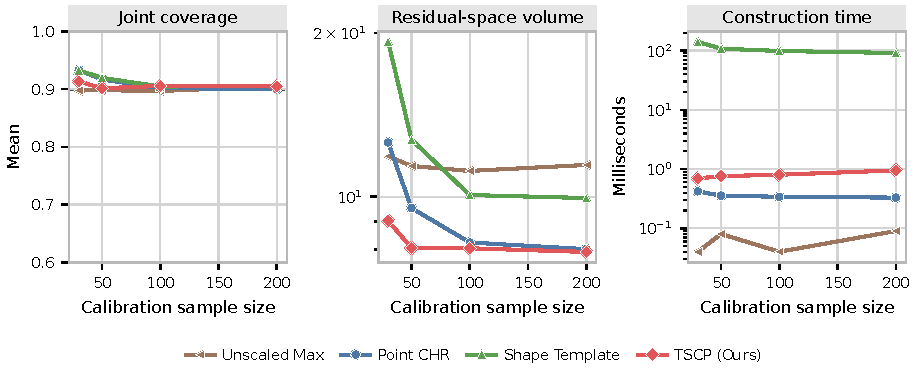
\includegraphics[width=0.92\textwidth]{figures/fig_app_shape_template_baseline.pdf}
  \caption{Comparison with a KDE/mean-shift hyperrectangular shape template
  for $d=2$ Gaussian residuals with scales $(2,1)$. Volume follows the same
  $2^{-d}$ normalization as the other residual-space experiments. Results
  average 100 independent repetitions. The shape-template method is slower and has larger volume than TSCP at every calibration size.}
  \label{fig:app-shape-template}
\end{figure*}

\FloatBarrier
\subsection{Oracle Approximation and Computational Scaling}
\label{app:ours_simulation}

We examine how the practical constructions approximate the population
oracle under independent Laplace noise with coordinate scales
$(d,d-1,\ldots,1)$ and varying calibration size.

The additional methods considered in this section include (i) \emph{Naive}, the heuristic plug-in rescaling method that uses location and scale parameters estimated directly from the calibration data without further adjustments, summarized in Algorithm~\ref{alg:std-plug-in}; (ii) \emph{TSCP-S}, the inefficient data-splitting variant summarized in Algorithm~\ref{alg:std-ds}; (iii) \emph{TSCP-GWC}, our conservative global-worst-case method summarized in Algorithm~\ref{alg:global}; (iv) \emph{TSCP-LWC}, the aggregated union described in Section~\ref{sec:method-lwc} but not enclosed by a rectangle.


\begin{figure}[!htbp]
    \begin{subfigure}[b]{\textwidth}
        \centering
        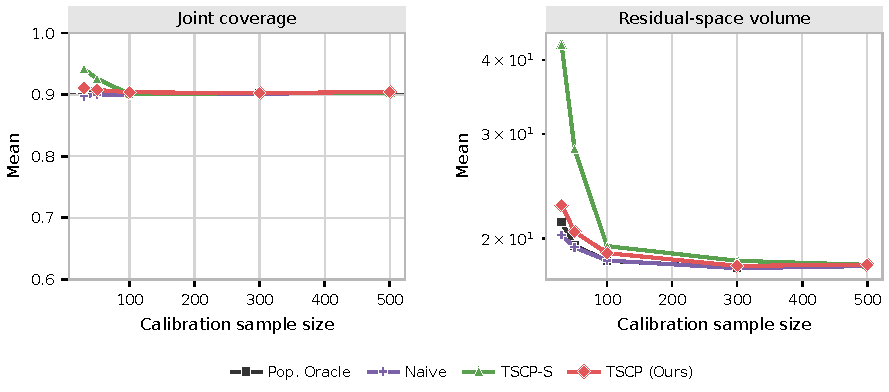
\includegraphics[width=0.9\textwidth]{figures/fig_app_oracle_approximation.pdf}
    \end{subfigure}
    \begin{subfigure}[b]{\textwidth}
        \centering
        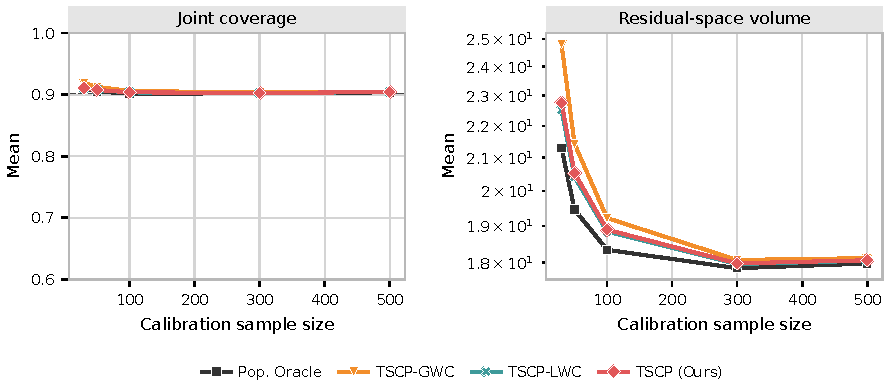
\includegraphics[width=0.9\textwidth]{figures/fig_app_local_enclosure_2d.pdf}
    \end{subfigure}
    \caption{Performance of TSCP and alternative approaches on simulated data with $d=2$ targets and heterogeneous Laplace noise. The target coverage level is $90\%$. Results are averaged over $200$ trials. All methods achieve near-nominal coverage and approximate \emph{Pop.~Oracle} as the calibration sample size increases. TSCP tracks TSCP-LWC closely, with an almost indistinguishable average volume, highlighting the tightness of its rectangular enclosure.}
    \label{fig:approximation1}
\end{figure}

The methods in Figure~\ref{fig:approximation1} approach the volume of
\emph{Pop.~Oracle} as $n$ increases. TSCP and TSCP-LWC have nearly
indistinguishable mean volumes, suggesting that the rectangular enclosure
adds little volume in this setting. TSCP-GWC is more conservative but
produces smaller volumes than the data-splitting variant TSCP-S. Despite
lacking a finite-sample coverage guarantee, the \emph{Naive} approach
performs well at larger calibration sizes, as also shown in
Figure~\ref{fig:approximation2}. Computational cost is examined separately below.

\begin{figure}[!htbp]
    \centering
    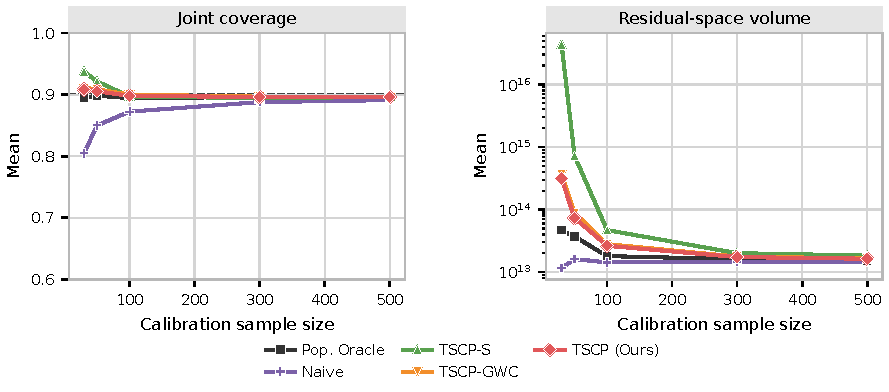
\includegraphics[width=0.9\textwidth]{figures/fig_app_local_enclosure_10d.pdf}
    \caption{Performance of TSCP and alternative approaches on simulated data with $d=10$ targets. Other details are as in Figure~\ref{fig:approximation1}. TSCP-LWC is omitted from this figure due to its prohibitive cost with even moderately high-dimensional outcomes.}
    \label{fig:approximation2}
\end{figure}

Figure~\ref{fig:runtime} better highlights the prohibitive computational cost of TSCP-LWC, by reporting on the results of similar experiments where a small sample size is fixed, $|\mathcal{D}_{\mathrm{cal}}|=30$, while the outcome dimensions are gradually increased: $d \in \{2, 3, 4, 5, 10, 20, 30\}$.

\begin{figure}[!htbp]
    \centering
    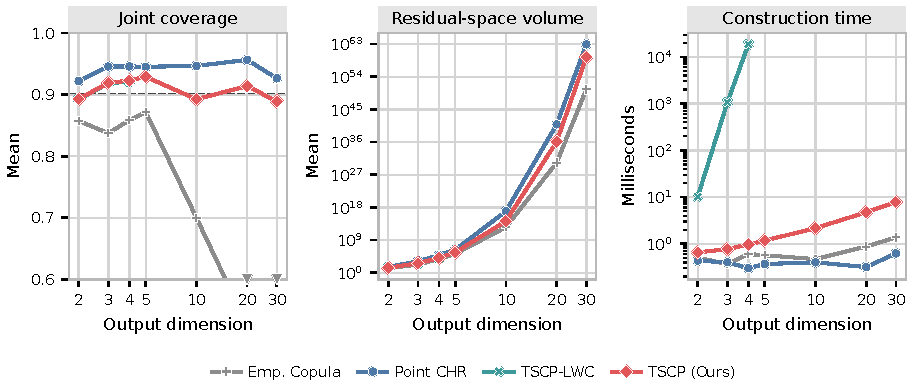
\includegraphics[width=\textwidth]{figures/fig_app_dimension_scaling.pdf}
    \caption{Absolute-residual experiment with Laplace noise, calibration
    size $n=30$, and varying output dimension $d$. Results are averaged
    over 30 repetitions. The dashed line marks target coverage $0.9$. TSCP-LWC is evaluated only at $d\in\{2,3,4\}$ because of
    its rapidly increasing computational cost.}
    \label{fig:runtime}
\end{figure}

\FloatBarrier
\subsection{Additional Real-Data Experiments}
\label{app:additional-real-experiments}

These diagnostics use 200 randomized splits per dataset with the same
allocation and model settings as Section~\ref{sec:real-data-experiments}.
All methods share the fitted model and observations within each split.
The reported variation is over splits of each fixed dataset, not over
independently sampled datasets from a population.

\subsubsection{Coordinate-Wise Marginal Coverage and Interval Lengths}
\label{app:real-coordinate-audit}
Figure~\ref{fig:real-marginal-coverage} reports coordinate-wise marginal coverage for each of the six real datasets. The dashed line indicates the target joint coverage of $0.9$, and each panel also reports TSCP's mean joint coverage. The coordinates follow the target-column order of each dataset, allowing for a clear comparison of how well each method performs across different dimensions of the outcome space.

\begin{figure}[!htbp]
  \centering
  
\includegraphics[width=0.96\textwidth]{figures/fig_app_real_marginal_coverage.pdf}
  \caption{Coordinate-wise marginal coverage over 200 splits of each
  real dataset. The dashed line is the $0.9$ joint target, and each panel
  also reports TSCP's mean joint coverage. Coordinates follow the target-column order of each dataset.}
  \label{fig:real-marginal-coverage}
\end{figure}

To compare
coordinate-wise lengths, Figure~\ref{fig:body-real-coordinate-bars}
reports the paired length ratio
\[
 A_{j,m}=\frac{1}{200}\sum_{r=1}^{200}
 \frac{\ell_{j,m}^{(r)}}{\ell_{j,\mathrm{Unscaled}}^{(r)}}.
\]
where $\ell_{j,m}^{(r)}=2\mathcal L_{j,m}^{(r)}$ is the full outcome-space
interval length for coordinate $j$, method $m$, and split $r$. 
Thus, a bar below one indicates a shorter interval on average relative to
Unscaled Max on the same splits. Ratios are formed before averaging; they
are not ratios of mean interval lengths. 

\begin{figure}[!htbp]
  \centering
  
\includegraphics[width=0.96\textwidth]{figures/fig_body_real_coordinate_bars.pdf}
  \caption{Coordinate-wise full interval lengths on all six real datasets,
  normalized within each split by the corresponding Unscaled Max length
  and then averaged over 200 splits. The dashed line marks a ratio of one.
  Point CHR is infinite on \texttt{stock}. These width comparisons should
  be read with the matching joint coverage and the marginal coverage in
  Figure~\ref{fig:real-marginal-coverage}.}
  \label{fig:body-real-coordinate-bars}
\end{figure}

\clearpage
\subsubsection{Backward-Search and Fallback Diagnostics}
\label{app:real-data-diagnostics}

We investigate the fallback and backward-search behavior of the TSCP
implementation summarized in Algorithm~\ref{alg:shortcut}. A fallback
occurs when the mean cell has empty intersection with the global rectangle;
a backward-search run occurs when that intersection is nonempty but the binary-search condition fails
for at least one coordinate. We also record the number of coordinates using
that branch and the number of candidate cells inspected before finding the boundary. 

Table~\ref{tab:real-search-diagnostics} reports the split-level and
coordinate-level counts. Figure~\ref{fig:real-search-diagnostics} shows the
number of candidate cells inspected per coordinate and the construction
time of the observed search regime. For each split, we time repeated TSCP
calls on the same calibration residuals after a warm-up. The mean of the
per-split median runtimes is
\[
\frac{1}{200}\sum_{s=1}^{200}
\operatorname{median}(T_{s1},\ldots,T_{sr}),
\]
where $T_{sj}$ is the runtime of the $j$th call on split $s$.
We use $r=7$ for $\alpha=0.1$ and $r=3$ for
$\alpha\in\{0.3,0.5,0.7,0.9\}$. These calls are repeated timing
measurements, not additional statistical repetitions. Regime-specific
times average the medians only over splits exhibiting that regime.
Timings exclude model fitting, residual computation, and diagnostic logging;
calls run serially with native thread pools limited to one thread.

\begin{table}[!htbp]
  \centering
  \scriptsize
  \setlength{\tabcolsep}{3pt}
  \begin{tabular}{lrrrrrrr}
\toprule
Dataset & $n$ & \shortstack{Backward\\splits} & \shortstack{Backward\\coordinates} & \shortstack{Fallback\\splits} & \shortstack{Binary only\\(ms)} & \shortstack{Any backward\\(ms)} & \shortstack{Fallback\\(ms)} \\
\midrule
\texttt{stock} & 15 & 0/200 & 0/1200 & 0/200 & 1.007 & -- & -- \\
\texttt{rf2} & 384 & 0/200 & 0/1600 & 0/200 & 2.780 & -- & -- \\
\texttt{scm1d} & 490 & 0/200 & 0/3200 & 0/200 & 7.239 & -- & -- \\
\texttt{scm20d} & 448 & 0/200 & 0/3200 & 0/200 & 7.120 & -- & -- \\
\texttt{energy} & 38 & 0/200 & 0/400 & 0/200 & 0.466 & -- & -- \\
\texttt{student} & 32 & 0/200 & 0/600 & 0/200 & 0.620 & -- & -- \\
\bottomrule
\end{tabular}

  \caption{Executed TSCP search regimes at target coverage $0.9$ on the
  six real datasets. Each split-count denominator is 200. The coordinate
  denominator is $d$ times the number of non-fallback splits. Conditional
  times summarize the full TSCP call, not just the backward loop; a dash
  denotes an unobserved regime. $n$ is the calibration size.}
  \label{tab:real-search-diagnostics}
\end{table}

\begin{figure}[!htbp]
  \centering
  
\includegraphics[width=0.96\textwidth]{figures/fig_body_real_search_diagnostics.pdf}
  \caption{TSCP search work and construction time for 200 splits
  per real dataset at target coverage $0.9$. Left: candidate cells inspected
  per coordinate, averaged over non-fallback runs. Counts include cells
  rejected by intersection checks. Right: construction times
  of the observed regime. Unobserved scenarios have no bars.}
  \label{fig:real-search-diagnostics}
\end{figure}

At the main target $\alpha=0.1$, neither backward search nor fallback occurs
in any of the 200 splits for any dataset. All 10,200 coordinate searches use
the binary branch, with about $4.00$--$8.49$ candidate-cell inspections per
coordinate on average across datasets. Observing no events in these splits
does not establish that backward search or fallback is impossible.

To explore further, we reuse the same 200
calibration residual matrices per dataset and vary the miscoverage level over
$\alpha\in\{0.1,0.3,0.5,0.7,0.9\}$. 
In this experiment, we observe that backward search and fallback occur more frequently at higher miscoverage levels.
On \texttt{energy} at $\alpha=0.5$, backward search occurs in $3/200$
splits ($1.5\%$), while fallback occurs in $140/200$ ($70\%$). The
remaining 57 splits use only binary search. At $\alpha=0.7$ and $0.9$, 10 energy splits use backward
search and 190 fall back. In every observed backward-search case, each of
the two coordinates inspects only \emph{one} backward candidate. 
No backward search
is observed in the other five datasets over the displayed levels.
Fallback is often faster because it returns the already computed global
rectangle, so a lower average runtime at an extreme target need not
indicate a more efficient local search. 

\begin{figure}[!htbp]
  \centering
  
\includegraphics[width=0.98\textwidth]{figures/fig_app_real_search_alpha.pdf}
  \caption{Computational stress test on the cached real-data calibration
  residuals. Each point summarizes 200 splits. The first two panels show
  the fractions of splits using any backward search or the global fallback. The final panel reports construction time.}
  \label{fig:app-real-search-alpha}
\end{figure}

\endgroup
